El algoritmo lleva el nombre de dos científicos estadounidenses: Richard Bellman y Lester Ford. De hecho, Ford inventó este algoritmo en 1956 durante el estudio de otro problema matemático, que eventualmente se redujo a un subproblema de encontrar los caminos más cortos en el grafo, y Ford dio un esquema del algoritmo para resolver este problema. Bellman en 1958 publicó un artículo dedicado específicamente al problema de encontrar el camino más corto, y en este artículo formuló claramente el algoritmo en la forma en que lo conocemos ahora.

A diferencia de muchos otros algoritmos de grafos, para el algoritmo de Bellman-Ford, es más 
conveniente representar el grafo usando una sola lista de todas las aristas (similar al algoritmo 
Kruskal) (en lugar de $n$ listas de adyacencia de cada vértice). Comenzamos la implementación con una 
estructura$\rm.arista$ para representar las aristas. La entrada al algoritmo son números. $n$ ,$m$ 
,lista $e$ de aristas y el vértice inicial $v$ . Todos los vértices están numerados de $1$ a $n$.

Si el grafo contiene un ciclo de coste negativo, el algoritmo lo detectará, pero no encontrará el 
camino más corto que no repite ningún vértice. La complejidad de este problema es al menos la del 
problema del camino más largo de complejidad NP-Completo.

El algoritmo de Bellman-Ford es, en su estructura básica, muy parecido al algoritmo de Dijkstra, 
pero en vez de seleccionar vorazmente el nodo de peso mínimo aun sin procesar para relajarlo, 
simplemente relaja todas las aristas, y lo hace $|V|-1$ veces, siendo $|V|$ el número de vértices en el grafo. Las repeticiones permiten a las distancias mínimas recorrer el árbol, ya que en la 
ausencia de ciclos negativos, el camino más corto solo visita cada vértice una vez. A diferencia 
de la solución voraz, la cual depende de la suposición de que los pesos sean positivos, esta 
solución se aproxima más al caso general.

Existen dos versiones:
\begin{itemize}
	\item Versión no optimizada para grafos con ciclos negativos, cuyo coste de tiempo es O(VE).
	\begin{lstlisting}[language=C++]
bool BellmanFord(Grafo G, nodo_origen s)
   // inicializamos el grafo. Ponemos distancias a INFINITO menos el nodo origen que 
   // tiene distancia 0
   for v in V[G] do
      distancia[v]=INFINITO
      predecesor[v]=NIL
   distancia[s]=0
   // relajamos cada arista del grafo tantas veces como numero de nodos -1 haya en el grafo
   for i=1 to |V[G]|-1 do
      for (u, v) in E[G] do
         if distancia[v]>distancia[u] + peso(u, v) then
            distancia[v] = distancia[u] + peso (u, v)
            predecesor[v] = u
   // comprobamos si hay ciclos negativo
   for (u, v) in E[G] do
     if distancia[v] > distancia[u] + peso(u, v) then
		print ("Hay ciclo negativo")
		return FALSE
   return TRUE
	\end{lstlisting} 
	\item Versión optimizada para grafos con aristas de peso negativo, pero en el grafo no existen 
	ciclos de coste negativo, cuyo coste de tiempo, es también O(VE). 
	\begin{lstlisting}[language=C++]
bool BellmanFord_Optimizado(Grafo G, nodo_origen s)
   // inicializamos el grafo. Ponemos distancias a INFINITO menos el nodo origen que
   // tiene distancia 0. Para ello lo hacemos recorriendonos todos los vertices del grafo
   for v in V[G] do
      distancia[v]=INFINITO
      padre[v]=NIL
   distancia[s]=0
   encolar(s, Q)
   en_cola[s]=TRUE
   while Q!=0 then
      u = extraer(Q)
      en_cola[u]=FALSE
      // relajamos las aristas
      for v in ady[u] do
         if distancia[v]>distancia[u] + peso(u, v) then
            distancia[v] = distancia[u] + peso (u, v)
            padre[v] = u
            if en_cola[v]==FALSE then
               encolar(v, Q)
               en_cola[v]=TRUE
	\end{lstlisting} 
\end{itemize}

El la siguiente imagen se muestra la ejcucción del algoritmo. El mismo comienza por el nodo z.

\begin{figure}[h]
	\centering 
	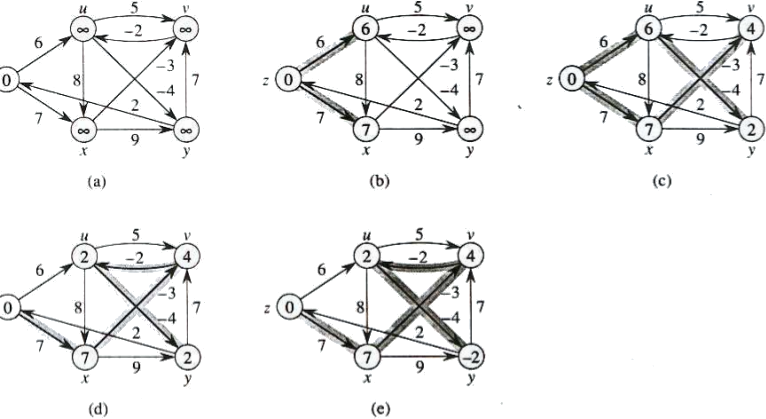
\includegraphics[scale=0.53]{img/bellman-ford}
	\caption{Ejecucción del algoritmo Bellman-Ford.}
	\label{contexto:figura6}
\end{figure}

\subsection{La prueba del algoritmo}

Primero, tenga en cuenta que para todos los vértices inalcanzables $u$ el algoritmo funcionará correctamente, la etiqueta $d[u]$ permanecerá igual al infinito (porque el algoritmo Bellman-Ford encontrará alguna forma de llegar a todos los vértices alcanzables desde el vértice inicial $v$ , y la relajación de todos los demás vértices restantes nunca ocurrirá).

Probemos ahora la siguiente afirmación: Después de la ejecución de $i_{th}$ fase, el algoritmo Bellman-Ford encuentra correctamente todos los caminos más cortos cuyo número de aristas no exceda $i$.

En otras palabras, para cualquier vértice $a$ denotemos la $k$ número de aristas en el camino más corto hacia él (si hay varios de esos caminos, puede tomar cualquiera). De acuerdo con esta declaración, el algoritmo garantiza que después de $k_{th}$ fase el camino más corto para el vértice $a$ será encontrado.

\textbf{Prueba}: Considere un vértice arbitrario $a$ al que hay un camino desde el vértice inicial 
$v$ , y considere un camino más corto hacia él $(p_0=v, p_1, \ldots, p_k=a)$. Antes de la primera 
fase, el camino más corto al vértice $p_0 = v$ fue encontrado correctamente. Durante la primera 
fase, la arista $(p_0,p_1)$ ha sido comprobada por el algoritmo, y por lo tanto, la distancia al 
vértice $p_1$ se calculó correctamente después de la primera fase. Repitiendo esta declaración $k$ veces, vemos que después $k_{th}$ fase la distancia al vértice $p_k = a$ se calcula correctamente, 
lo que queríamos probar.

Lo último que hay que notar es que cualquier camino más corto no puede tener más de $n - 1$ bordes Por lo tanto, el algoritmo sube lo suficiente a la $(n-1)_{th}$ fase. Después de eso, se garantiza que ninguna relajación mejorará la distancia a algún vértice.

\subsection{Ruta de recuperación}

Consideremos ahora cómo modificar el algoritmo para que no solo encuentre la longitud de los caminos más cortos, sino que también permita reconstruir los caminos más cortos.

Para eso, vamos a crear otro arreglo $p[1 \ldots n]$, donde para cada vértice almacenamos su predecesor, es decir, el penúltimo vértice en el camino más corto que conduce a él. De hecho, el camino más corto a cualquier vértice $a$ es un camino más corto a algún vértice $p[a]$, a lo que añadimos $a$ al final del camino.

Tenga en cuenta que el algoritmo funciona con la misma lógica: asume que la distancia más corta a un vértice ya está calculada e intenta mejorar la distancia más corta a otros vértices desde ese vértice. Por lo tanto, a la hora de mejorar solo debemos recordar $p[]$, es decir, el vértice a partir del cual se ha producido esta mejora.

\subsection{El caso de un ciclo negativo}

En todo lo anterior, consideramos que no hay un ciclo negativo en el grafo (precisamente, nos interesa un ciclo negativo que sea alcanzable desde el vértice inicial $v$, y, para ciclos inalcanzables, no cambia nada en el algoritmo anterior). En presencia de un ciclo o ciclos negativos, existen otras complicaciones asociadas con el hecho de que las distancias a todos los vértices de este ciclo, así como las distancias a los vértices alcanzables desde este ciclo, no están definidas: deben ser iguales a menos infinidad $(-\infty)$.

Es fácil ver que el algoritmo de Bellman-Ford puede hacer la relajación sin fin entre todos los vértices de este ciclo y los vértices alcanzables desde él. Por lo tanto, si no limita el número de fases a $n-1$ , el algoritmo se ejecutará indefinidamente, mejorando constantemente la distancia desde estos vértices. De ahí obtenemos el \textbf{criterio de presencia de un ciclo de pesos negativos alcanzable para el vértice fuente} $v$: después $(n-1)_{th}$ fase, si ejecutamos el algoritmo para una fase más, y realiza al menos una relajación más, entonces el gráfico contiene un ciclo de peso negativo al que se puede acceder desde $v$; de lo contrario, tal ciclo no existe.

Además, si se encuentra dicho ciclo, el algoritmo de Bellman-Ford puede modificarse para que 
recupere este ciclo como una secuencia de vértices contenidos en él. Para ello es suficiente 
recordar el último vértice $x$ por lo que hubo una relajación en $n_{th}$ fase. Este vértice estará 
en un ciclo de peso negativo o será accesible desde él. Para obtener los vértices que están 
garantizados para estar en un ciclo negativo, comenzando desde el vértice $x$, pasar a los 
predecesores $n$ veces. Por lo tanto obtendremos el vértice $y$, es decir, el vértice en el ciclo 
más temprano accesible desde la fuente. Tenemos que ir desde este vértice, a través de los 
predecesores, hasta volver al mismo vértice $y$ (y sucederá, porque la relajación en un ciclo de 
peso negativo ocurre de manera circular).